\section{Preliminary} \label{sec:prelim}

\subsection{STT-RAM Cell Basics} 
STT-RAM uses MTJ as the memory storage and leverages the difference in magnetic directions to represent the memory bit.  As shown in Fig.~\ref{fig:mram_cell}, MTJ usually contains two ferromagnetic layers.  One ferromagnetic layer is has fixed magnetization direction and it is called the reference layer, while the other layer has a free magnetization direction that can be changed by passing a write current and it is called the free layer. The relative magnetization direction of two ferromagnetic layers determines the resistance of MTJ.  If two ferromagnetic layers have the parallel directions, the resistance of MTJ is low, indicating a ``1" state; if two layers have anti-parallel directions, the resistance of MTJ is high, indicating a ``0" state.

As shown in Fig.~\ref{fig:stt_cell}, there are two possible schemes to stack MTJ atop access NMOS transistor. Conventionally, the free layer of MTJ is connected to bitline~(BJ). In that scheme, when writing ``1" state into STT-RAM cells, positive voltage difference is established between BL and SL and the switching current required is $I_{c}(AP\rightarrow P)$; when writing ``0" state, negative voltage difference is established between BL and SL and the switching current required is $I_{c}(P\rightarrow AP)$. While the reverse connection scheme was proposed in~\cite{STTRAM:Qualcomm09} where the free layer of MTJ is connected to the drain of NMOS instead of BL. \cite{STTRAM:Qualcomm09} argues that $I_{c}(P\rightarrow AP)$ is normally significantly larger than $I_{c}(AP\rightarrow P)$~/cite{STTRAM:APL05,STTRAM:PRB05} due to the inherent torque asymmetry of MTJ. But the SL-to-BL current is much smaller than the BL-to-SL current under the same wordline voltage and voltage difference between BL and SL because the body effect of access transistor degrades the SL-to-BL current remarkably. Thus reserving connection scheme can relax the sizing requirement on access transistor, which results in more compact STT-RAM cell size. However, device-level efforts have been put to improve the asymmetry of switching characteristic of MTJ and $I_{c}(AP\rightarrow P)$ slightly larger than $I_{c}(P\rightarrow AP)$ was even demonstrated in~\cite{STTRAM:Grandis07}. In our work, we always choose the MJT connection scheme that is responsible for relaxed sizing requirement on access transistor.

\begin{figure}[t]
  \centering
  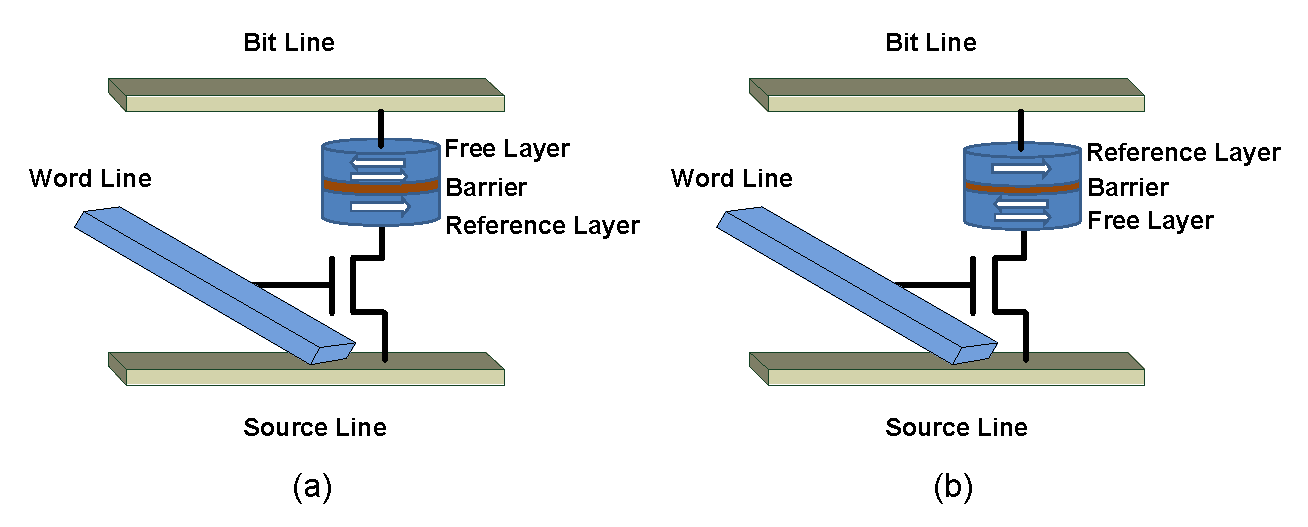
\includegraphics[width=3.5in]{fig/sttramcell.eps}
  \caption{Demonstration of a STT-RAM cell: (a) Conventional connection scheme; (b) Reverse connection scheme.}
  \label{fig:stt_cell}
\end{figure}


\subsection{Write current versus write pulse width trade-off} 
The current amplitude required to reverse the direction of the free ferromagnetic layer is determined by the size and aspect ratio of MTJ and the write pulse duration.

Generally, the smaller the MTJ is or the longer the write pulse is applied, the less the critical switching current is needed to switch the MTJ state.

